%! root = thesis.tex

\chapter{\label{ch:1-intro}Introduction}

The construction of modern software relies on an ever-growing ecosystem of technologies and towers of abstraction.
Contemporary systems integrate dozens of third-party libraries, span multiple programming languages, and depend on countless layers of middleware and hardware interfaces.
Modern web browsers, for example, consist of 20 or even 30 million lines of code~\cite{openhub-firefox,openhub-chromium}.
While this ecosystem enables developers to build software systems of unprecedented functionality, the increasing complexity also creates new challenges.

Despite this rise in complexity, the core expectations of software have remained unchanged: it is supposed to be secure, correct, reliable, and efficient.
Yet, as systems grow, these qualities become harder to maintain and are often in tension with one another.
Each new abstraction layer, for example, hides details but also introduces uncertainty about the layer below.
Likewise, performance optimization risks new corner cases, and each extension of functionality opens new attack surfaces.
Catastrophic security breaches like Heartbleed~\cite{heartbleed} (a simple buffer over-read in a core library), Spectre~\cite{Kocher2019} (exploiting CPU-level speculation), or Log4Shell~\cite{log4shell} (a failure in input sanitization) --- each with global consequences --- show that these problems are not just hypotheticals.

Similarly, reliability failures like silent miscompilations have plagued even widespread production compilers such as GCC and LLVM \cite{yang2011,wang2012}.
\citeauthor{yang2011} showed that the \propername{Csmith} fuzzer alone uncovered more than 325 previously unknown bugs in GCC and LLVM, including release-blocking miscompilations~\cite{yang2011}.
Subsequent longitudinal analyses of hundreds of LLVM and GCC bug reports find that miscompilations continue to account for a large fraction of confirmed issues and often remain latent for months before being diagnosed~\cite{chen2016}.
Recent work also showed that bugs in the compiler not only threaten the reliability of the compiled software, but can also introduce security bugs~\cite{xu2023a,Xu2023}.

These data points underline that both the software we deploy and the toolchains we depend on remain fragile in practice.
Thus, security and reliability form two sides of the broader struggle for software \emph{trustworthiness}: the ability to rely on software to uphold its specification under \emph{both} benign and adversarial conditions.
The quest for software trustworthiness is not new.
Despite decades of academic research and industrial mitigation efforts, however, challenges in software security and reliability remain, not least because the complexity of software keeps growing.
The following sections analyze in more detail why security and reliability are no \enquote{solved problems} yet.


\section{Security}
The tradeoff between abstraction and performance explains, in part, why languages like C or \cpp still form the foundation of critical infrastructure.
The potential for high performance\footnote{Not every program written in C or \cpp is automatically fast.} and direct control of machine internals make C and \cpp popular choices for operating systems, browsers, and embedded systems.
However, C and \cpp are also notorious for their lack of automatic memory management (memory unsafety) and, more broadly, for the pitfalls of undefined behavior.

These pitfalls regularly lead to dangerous vulnerabilities.
These vulnerabilities---which include both spatial (\eg buffer and heap overflows) and temporal memory safety (\eg use-after-free) issues---are the vector for a majority of remote code execution exploits.
Industry telemetry highlights the breadth of the problem.
In 2019, Microsoft’s Security Response Center reported that roughly 70\% of the critical vulnerabilities it handled over the past decade were due to memory-safety errors, despite major investments in defensive coding practices~\cite{msrcreport2019}.
Google’s annual Android security review reaches similar conclusions, attributing more than three quarters of high-severity platform bugs between 2019 and 2022 to memory-safety violations, many rooted in native code dependencies\cite{projectzeroandroid2022}.
Google's Project Zero also notes that the majority of the 2023 zero-days they investigated ultimately stemmed from memory corruption~\cite{projectzerointhewild2024}.

The rise in security-awareness and with it the increasing adoption of memory-safe languages also for system-related tasks is a welcome development.
Nonetheless, despite the rise of languages like Rust, C and \cpp remain dominant, consistently ranking in the top tiers of language popularity indices~\cite{tiobe2025}.
Furthermore, even new, memory-safe code is often integrated into legacy systems.
A vulnerability in an underlying C library, for example, can be exploited to undermine the guarantees of a Rust or Swift application that links against it~\cite{mergendahl2022}.
Even if from now no new code was written in memory-unsafe languages, migrating the billions of lines of C and \cpp code already in production would be a multi-year enterprise costing billions of euros.
Thus, memory safety vulnerabilities will remain a critical threat in the foreseeable future and mitigations are needed to deal with them.


\begin{figure}[t]
    \centering
    \resizebox{\textwidth}{!}{% code / cfi / randomization
% Data from DBLP cache
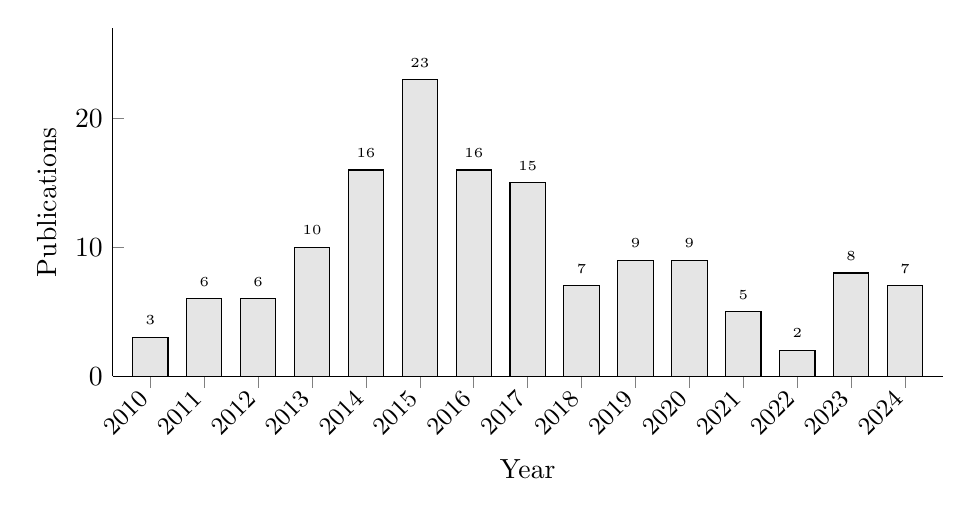
\begin{tikzpicture}
\begin{axis}[
    ybar,
    bar width=0.45cm,
    width=\textwidth,
    height=6cm,
    xlabel={Year},
    ylabel={Publications},
    ymin=0,
    ymax=27,
    xtick={2010,2011,2012,2013,2014,2015,2016,2017,2018,2019,2020,2021,2022,2023,2024},
    xticklabel style={rotate=45, anchor=east, font=\small, /pgf/number format/1000 sep={}},
    nodes near coords,
    nodes near coords style={font=\tiny, above},
    every node near coord/.append style={yshift=1pt},
    axis lines*=left,
    enlarge x limits=0.05,
]
\addplot[fill=gray!20, draw=black, line width=0.4pt] coordinates {
    (2010, 3)
    (2011, 6)
    (2012, 6)
    (2013, 10)
    (2014, 16)
    (2015, 23)
    (2016, 16)
    (2017, 15)
    (2018, 7)
    (2019, 9)
    (2020, 9)
    (2021, 5)
    (2022, 2)
    (2023, 8)
    (2024, 7)
};
\end{axis}
\end{tikzpicture}}
    \caption{Code-reuse attack and defense publications in security venues (IEEE S\&P, USENIX Security, CCS, NDSS, AsiaCCS, Euro S\&P) from 2010 to 2024.
    The paper metadata was retrieved from DBLP, and filtered using semantic clustering on titles and abstracts.
    The full list of papers is provided in \Cref{app:code-reuse-papers}.}
    \label{fig:intro:code-reuse-trend}
\end{figure}

A dominant class of exploits targeting these vulnerabilities is code-reuse attacks.
Attackers hijack a program's control flow and subsequently reuse existing code \enquote{gadgets} already present in the target process.
This approach allows attackers to bypass defenses like \wox, which, thanks to widespread hardware support, have become a de facto standard.
Over the years, different ways of defending against this type of attack have emerged.
One prominent defense category is randomization or more broadly, software diversity.
Software diversity embraces the possibility of memory corruptions and control-flow diversion and instead aims to restrict an attacker's mobility.
By introducing controlled randomness into code or data layouts, software diversity disrupts attackers’ assumptions.
For example, without knowing the exact location of functions or gadgets, an attacker can no longer use them in a code-reuse attack.
Unfortunately, closing all information channels an attacker could use to undermine the guarantees provided by randomization proves difficult in practice.
Recent work shows that even when code is perfectly hidden, predictable data structures such as the stack, global objects, or allocator metadata, can leak enough information for a successful attack~\cite{Rudd2017}.
The consequence is that although, judging by the publication counts, the security community's interest in code-reuse mitigations has declined, unsolved problems remain.
\Cref{fig:intro:code-reuse-trend} shows the number of code-reuse-related publications in top security venues from 2010 to 2024.
The figure clearly shows the peak interest around 2015--2016 and the subsequent decline.
While hardware defenses like Intel CET and ARM PAC have reduced the urgency for software-only solutions, they are not a silver bullet and research continues, particularly for embedded systems and attestation.
This trend is particularly worrying given the rapidly increasing capabilities of \gls{LLM}s with respect to offensive security.
Already in the year 2026, \gls{LLM}s can reduce the cost of creating highly sophisticated code-reuse exploits from days or even weeks down to a few hours and an investment of a few euros, and this is likely only the beginning~\cite{anthropic2026zerodays}.
At these drastically reduced costs, even sophisticated targeted attacks fall within the capabilities of non-state actors.
In light of these developments, we hope that the loss of interest in \glspl{CRA} is only temporary and that research on more capable defenses continues.
\section{Reliability}
Traditional approaches to software reliability, such as static analysis, unit testing, and formal verification, serve as the foundation of quality assurance.
While formal verification offers the strongest theoretical guarantees, it faces significant practical hurdles.
A key problem is often the lack of specification: verification requires properties to be formally defined, yet formulating such specifications is usually non-trivial.
Even when adequate specifications exist, the computational cost and limited scalability of formal methods prove prohibitive for large, evolving systems.
Similarly, static analysis faces inherent trade-offs between precision and scalability.
Finally, unit testing remains the most widespread technique but suffers from a critical blind spot: it is conceptually limited by human foresight and can only validate scenarios explicitly anticipated by the test author.

In light of these shortcomings, a long-neglected technique named fuzz testing, or fuzzing for short, has become increasingly important over the past 10--15 years.
This rise in popularity happened partly because of \propername{AFL}, a practical and fast fuzzer that combines code coverage feedback with carefully engineered heuristics.
Early fuzzers mostly relied on simple, random input generation and were often dismissed as crude or ad hoc.
Modern fuzzing, by contrast, combines feedback-guided input mutation and scheduling, constraint solving, and domain-specific generators to explore program behaviors more systematically.
Industrial-strength frameworks such as \aflpp, \propername{libFuzzer}, and their successors have demonstrated that fuzzing can uncover deep, previously unknown bugs in widely deployed software, including operating systems, browsers, cryptographic libraries, and compilers.

Most popular fuzzers like \aflpp and \propername{libFuzzer} rely on code coverage feedback to guide their mutation and scheduling decisions.
Despite its widespread use, code coverage is an imperfect proxy for test effectiveness, particularly for state-rich systems such as compilers.
Code coverage metrics---statement, branch, or edge coverage---abstract away the program’s internal state and treat all executions that follow the same control-flow paths as equivalent.
As a result, fuzzers can quickly saturate coverage while still failing to explore nuanced interactions within the same control-flow.
To find these deeper bugs, the fuzzer needs a better guide---one that considers more of the target program's internal state space.

%Meanwhile, the tools we use to build everything else—modern compilers, linkers, and virtual machines—have themselves grown complexity.
%Each new optimization pass, hardware backend, or language front-end enlarges the space of subtle interactions that manual review or unit tests rarely exercise, so bugs continue to slip through release pipelines.
%These observations are particularly true for \glspl{JIT}.
%\glspl{JIT} are typically part of a language VM and compile user-provided, potentially malicious code.
%When compiling such code, \glspl{JIT} are supposed to upkeep the sandboxing guarantees of the underlying language VM, such as enforcing array boundaries.
%As such, the correctness of \glspl{JIT} has an important security dimension as well.
%

\section{The Compiler's Role Beyond Optimization}
In this thesis I argue that compilers are uniquely positioned to help improve both software reliability and security.
Every non-trivial program passes through a compiler at some point, either ahead of time or just in time\footnote{Interpreted programs are an exception, but the interpreter itself has passed through a compiler as well.}.
Due to this compilation \enquote{bottleneck}, a single transformation deployed in the toolchain can harden millions of downstream binaries.

Compilers possess semantic insight that is hard, if not impossible, for post-compilation transformations to replicate.
The compiler's knowledge encompasses both programming language semantics and details about the target machine.
Compilers, for example, know the exact type hierarchy of compiled \cpp programs and the exact geometry of their stack frames.
While this information can be partially recovered from binaries, the reconstruction is notoriously challenging because compilation is a lossy process.
Similarly, compilers have detailed knowledge about the compilation process itself, such as which transformations were applied and which invariants justified those transformations.

In this thesis I explore how to tap these information sources for security hardening and improved fuzzing feedback.

\section{Structure}

This thesis presents three contributions that demonstrate the compiler's potential to improve software security and reliability.
The common thread is the compiler's unique vantage point: it possesses semantic knowledge about program structure that can be leveraged for purposes \emph{beyond optimization}.
The contributions are structured into two parts, with \cref{part:defense} focusing on security and \cref{part:fuzzing} on fuzzing.
Each part concludes with an \emph{Outlook} chapter that discusses more general ideas and possible future research directions.

\paragraph{R2C: Compiler-Driven Data Diversity}
In \cref{ch:r2c} I present \rtwoc, a novel software diversity defense that addresses the challenge of layout inference through information leaks.
Unlike prior work that focused primarily on code randomization, \rtwoc leverages the compiler's knowledge of stack frame geometry to randomize observable data layouts.
By disguising sensitive pointers among booby-trapped decoys, \rtwoc substantially raises reconnaissance cost while incurring moderate performance overhead.
While introducing new diversity techniques, \rtwoc also reveals the challenges diversity faces when subjected to targeted attacks with a powerful threat model.

\paragraph{LOOL: Optimization-Aware Compiler Fuzzing}
In \cref{ch:lool} I present \lool, a compiler fuzzing framework based on a new type of coverage feedback.
Instead of relying on code coverage, \lool leverages the compiler's own optimization log as a domain-specific feedback signal.
A genetic algorithm uses this feedback to steer test-case generation toward rare optimization interactions that are difficult to trigger otherwise.
Our suggested domain-specific coverage is both more efficient and targeted than code coverage.

\paragraph{Program State Projection}
In \cref{ch:psp} I present \emph{Program State Projection} (PSP), a technique that uses compiler analyses to expose hidden data dependencies to coverage-guided fuzzers.
By transforming indirect calls into explicit control-flow branches and partitioning value ranges, PSP aims to provide stepping stones that help fuzzers explore program states that conventional coverage metrics would conflate.
Although at present our evaluation shows no quantifiable gains in terms of code coverage and bug-finding performance, the broader \gls{PSP} framework reveals a new principle for supporting code-coverage-guided fuzzers.
